% Latex template: mahmoud.s.fahmy@students.kasralainy.edu.eg
% For more details: https://www.sharelatex.com/learn/Beamer

\documentclass{beamer}					% Document class
\geometry{papersize={15cm,10cm}}

\setbeamertemplate{footline}[text line]{%
  \parbox{\linewidth}{\vspace*{-8pt}\hfill\hfill\insertpagenumber}}
\setbeamertemplate{navigation symbols}{}

\usepackage[english]{babel}				% Set language
\usepackage[utf8x]{inputenc}			% Set encoding

\mode<presentation>						% Set options
{
  \usetheme{default}					% Set theme
  \usecolortheme{default} 				% Set colors
  \usefonttheme{default}  				% Set font theme
  \setbeamertemplate{caption}[numbered]	% Set caption to be numbered
}

% Uncomment this to have the outline at the beginning of each section highlighted.
%\AtBeginSection[]
%{
%  \begin{frame}{Outline}
%    \tableofcontents[currentsection]
%  \end{frame}
\usepackage{graphicx}					% For including figures
\usepackage{booktabs}					% For table rules
\usepackage{hyperref}	
\usepackage{tikz-network}				% For cross-referencing
\usepackage[absolute,overlay]{textpos}
\usepackage{bm}
\usepackage[font=small,labelfont=bf]{caption}				% For cross-referencing
\usepackage{comment}

\title{Visualizing nucleosome cluster dynamics with dense single molecule localization microscopy}	% Presentation title
\author{Clayton W. Seitz}								% Presentation author
\date{\today}									% Today's date	

\begin{document}

% Title page
% This page includes the informations defined earlier including title, author/s, affiliation/s and the date
\begin{frame}
  \titlepage
\end{frame}


% The following is the most frequently used slide types in beamer
% The slide structure is as follows:
%
%\begin{frame}{<slide-title>}
%	<content>
%\end{frame}


\begin{frame}
\begin{itemize}
\item Overview of biological system and some literature review
\item Open questions in that system
\item A novel method to study that system
\item Major results so far
\item Future goals and perspectives
\end{itemize}
\end{frame}


\begin{frame}{A phase separation model for transcriptional control}

\begin{textblock*}{6cm}(0.5cm,1.5cm)
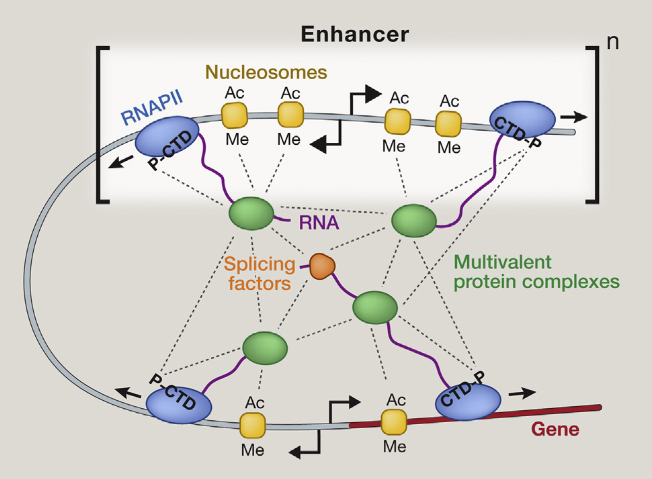
\includegraphics[width=6cm]{Super1.png}
\end{textblock*}

\begin{textblock*}{6cm}(6.75cm,1.5cm)
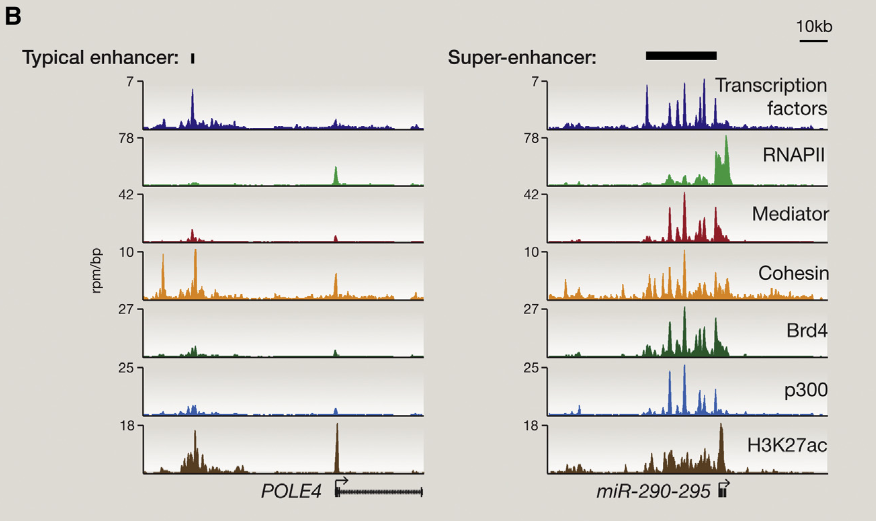
\includegraphics[width=7.4cm]{Super2.png}
\end{textblock*}

\begin{textblock*}{14cm}(0.5cm,6.5cm)
\textit{Hnisz et al. A phase separation model of transcriptional control. Cell 2017}
\end{textblock*}

\begin{textblock*}{14cm}(0.5cm,7.5cm)
\begin{itemize}
\item Super-enhanced genes are regulated by large molecular assemblies
\item BRD4 is an interesting target since specific and non-specific inhibitors exist
\item Nucleosome organization is poorly characterized at super-enhancers
\end{itemize}
\end{textblock*}

\end{frame}



\begin{frame}{(+)-JQ1 in complex with BRD4 protein}

\begin{textblock*}{6cm}(1.0cm,1.5cm)
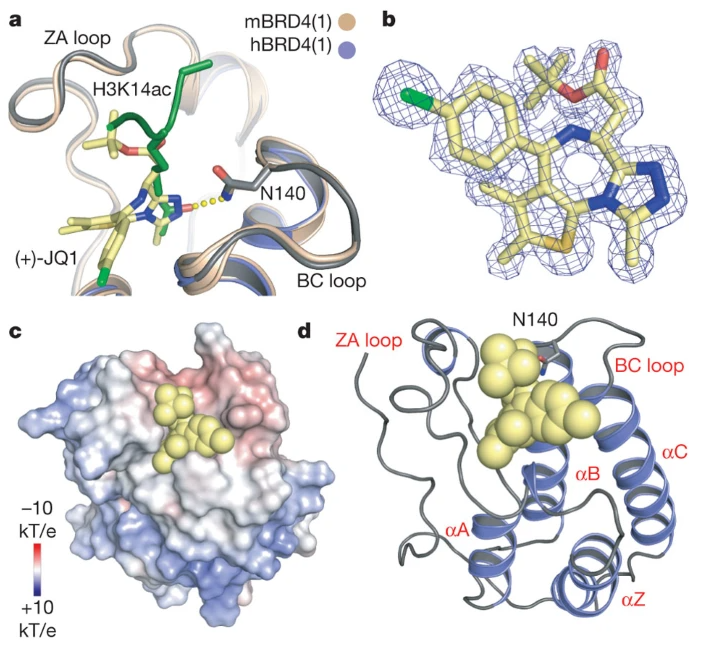
\includegraphics[width=6cm]{JQ1_Complex.png}
\end{textblock*}

\begin{textblock*}{8cm}(7.5cm,1.75cm)
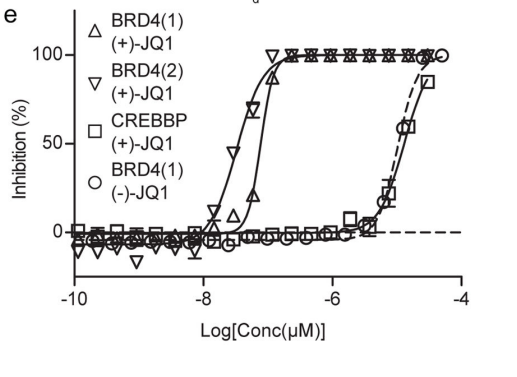
\includegraphics[width=8cm]{BRD4-Inhibition.png}
\end{textblock*}

\begin{textblock*}{\textwidth}(1.0cm,7.5cm)
\textit{Filippakopoulos. Selective inhibition of BET bromodomains. Nature }

\begin{textblock*}{14cm}(0.5cm,8.25cm)
\begin{itemize}
\item BRD4 has disordered domains which are thought to promote phase separation
\item Non-specific phase separation inhibitors exist
\end{itemize}
\end{textblock*}

\end{textblock*}


\end{frame}


\begin{frame}{Inhibition of a super-enhanced gene with JQ1}
\begin{figure}
\includegraphics[width=13cm]{GBP5-1.png}
\end{figure}
\begin{itemize}
\item Blue - DAPI (binds DNA minor groove)
\item White arrows highlight putative GBP5 transcription sites
\end{itemize}
\end{frame}

\begin{frame}{Inhibition of a super-enhanced gene with JQ1}
\begin{figure}
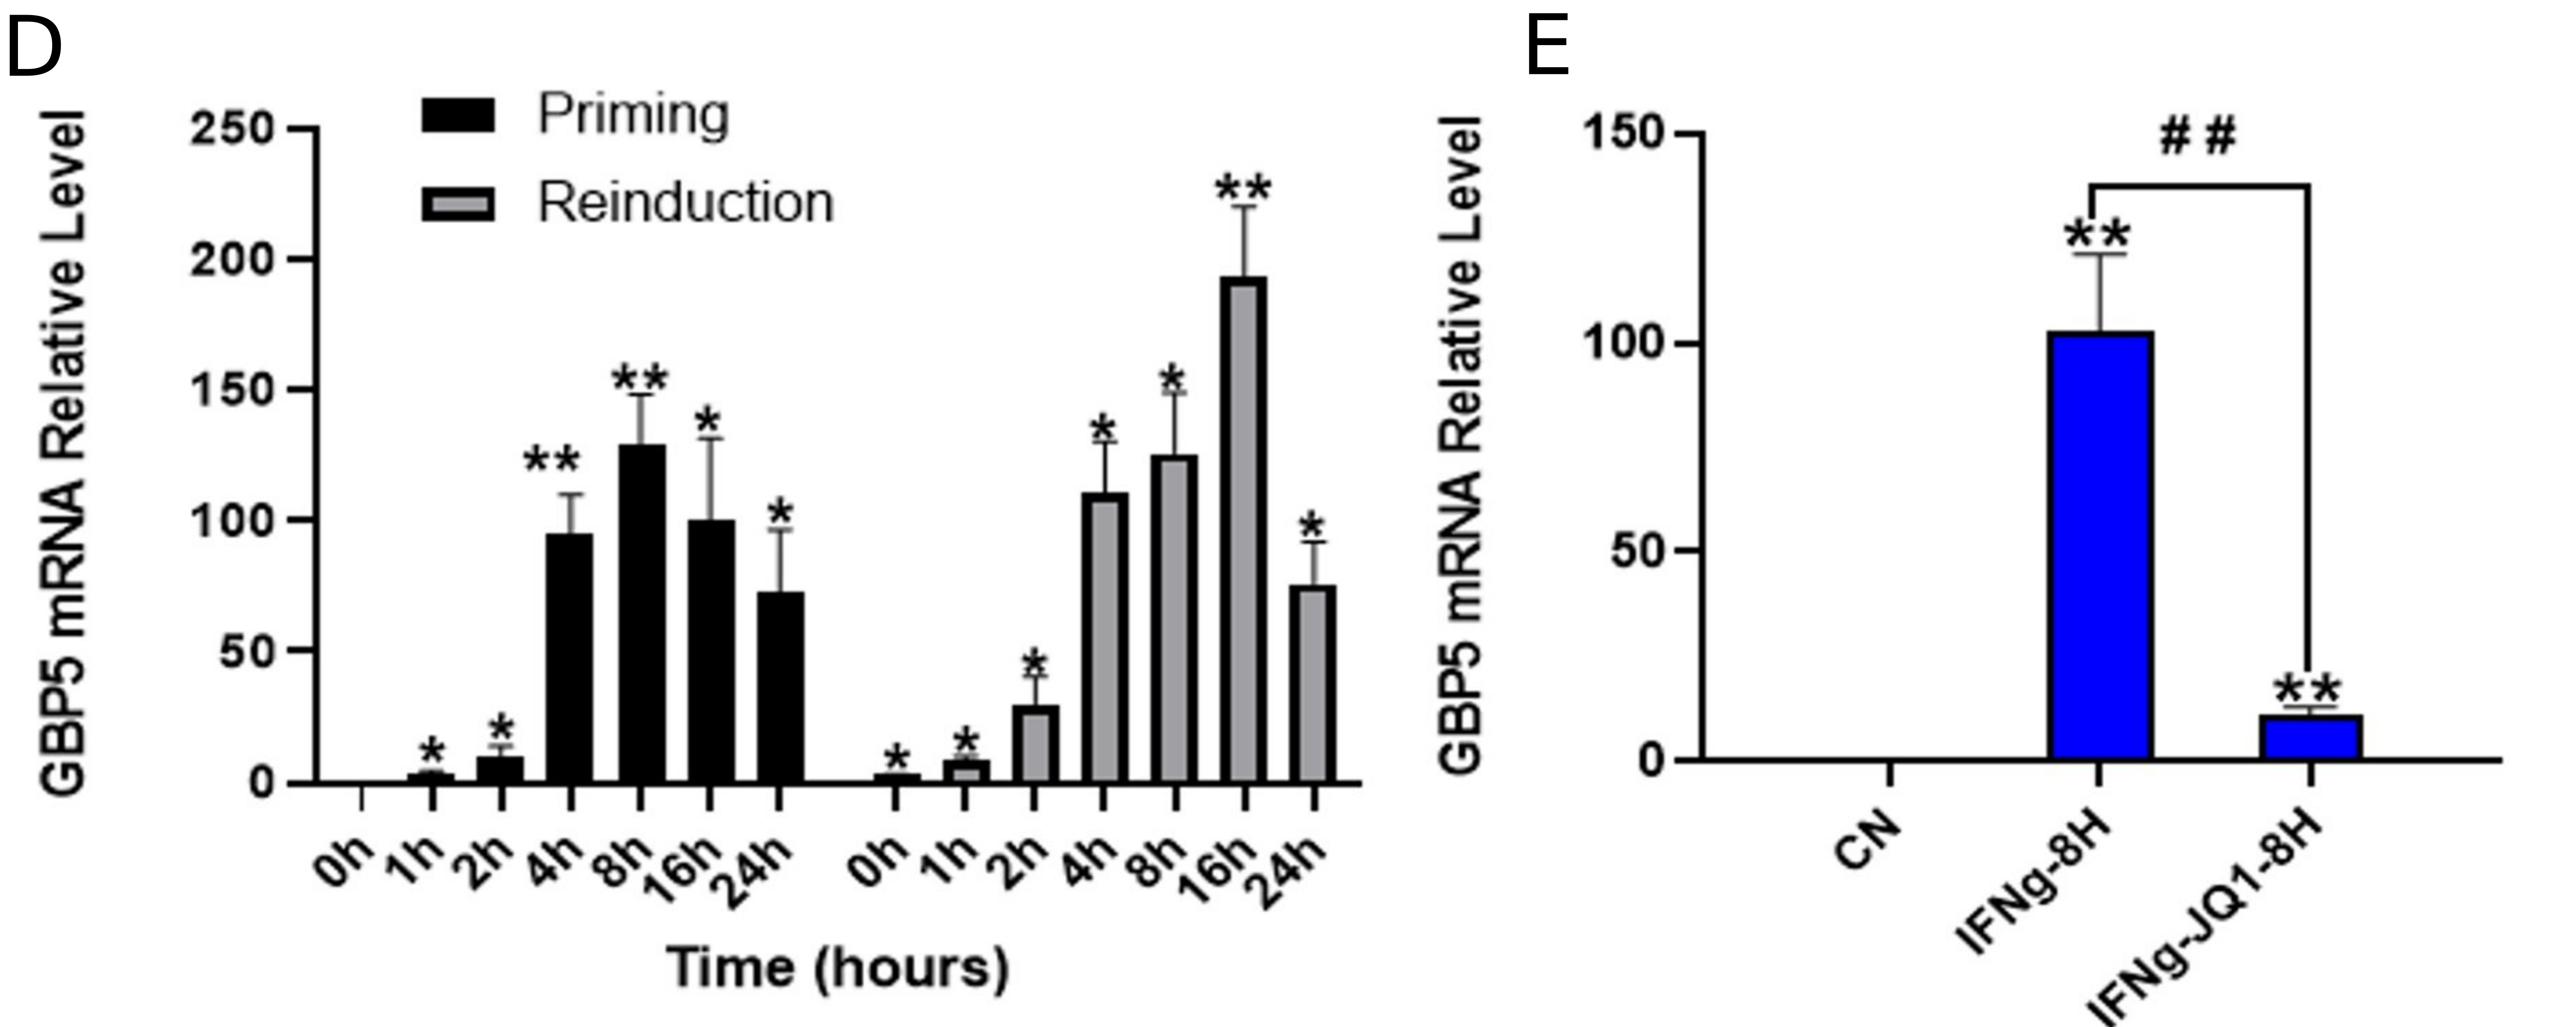
\includegraphics[width=12cm]{GBP5-2.png}
\end{figure}
\begin{itemize}
\item *:$P \leq 0.1$, **:$P \leq 0.01$
\end{itemize}
\end{frame}


\begin{frame}
\frametitle{Instrumentation for single molecule localization microscopy}

\begin{figure}
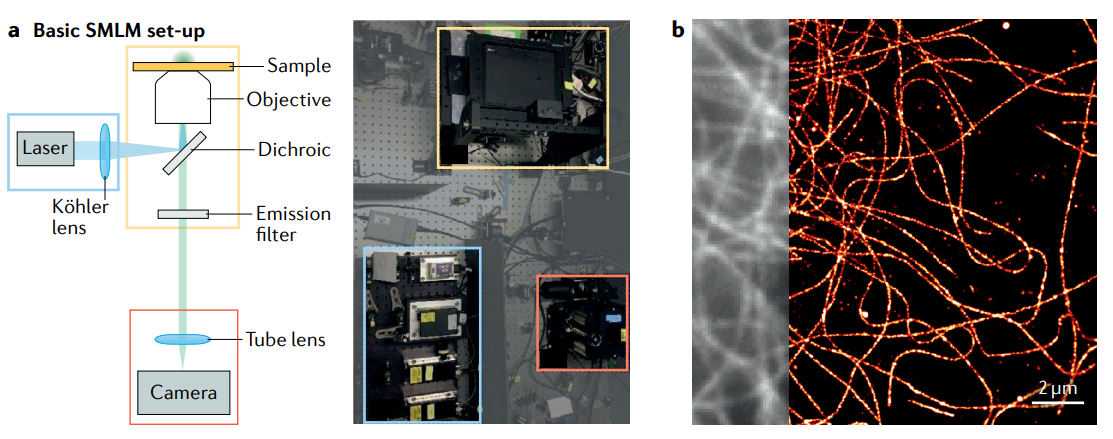
\includegraphics[width=12cm]{Setup.png}
\end{figure}

\end{frame}

\begin{frame}{A Poisson approximation at moderate SNR simplifies SMLM}

\begin{figure}
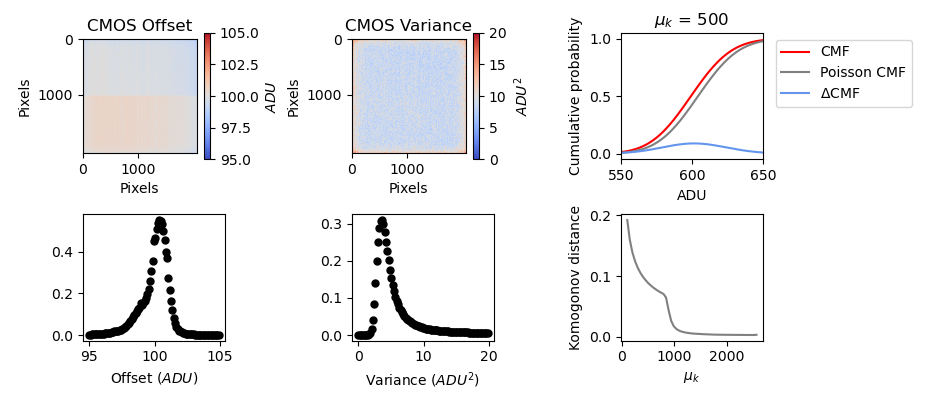
\includegraphics[width=13cm]{Noise.png}
\end{figure}

\begin{equation*}
P(H_{k}|\theta) = A\sum_{q=0}^{\infty} \frac{1}{q!}e^{-\mu_{k}}\mu_{k}^{q}\frac{1}{\sqrt{2\pi}\sigma_{k}}e^{-\frac{(H_{k}-g_{k}q-o_{k})}{2\sigma_{k}^{2}}}
\end{equation*}

$P(H_{k}|\theta)$ can be approximated as Poisson at high signal-to-noise ($\mathrm{SNR}$)
 
\end{frame}

\begin{comment}
\begin{frame}{Maximum likelihood localization of an isolated fluorescent emitter}
Localization: $\theta^{*} = \underset{\theta}{\mathrm{argmax}}\prod_{k}P(H_{k}|\theta)= \underset{\theta}{\mathrm{argmin}}-\sum_{k}\log P(H_{k}|\theta)$

\begin{textblock*}{8cm}(6.5cm,2.5cm)
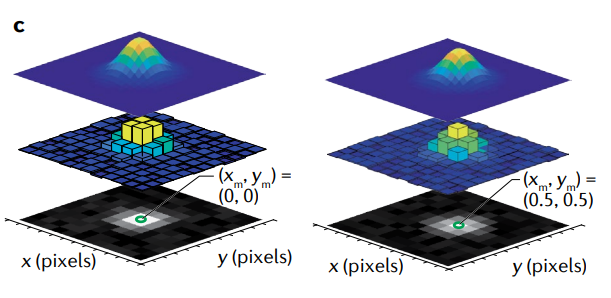
\includegraphics[width=\textwidth]{Model.png}
\end{textblock*}

\begin{textblock*}{2cm}(1cm,2.5cm)
\begin{align*}
\mu_{k} &= g_{k}\textcolor{red}{\eta} \textcolor{cyan}{N_{0}}\textcolor{blue}{\Delta}\int_{\mathrm{pixel}} G(x,y)dA\\
\\
\textcolor{red}{\eta} &- \mathrm{quantum\; efficiency}\\
\textcolor{cyan}{N_{0}} &- \mathrm{photon\; count}\\
\textcolor{blue}{\Delta} &- \mathrm{exposure\; time}
\end{align*}
\end{textblock*}



\vspace{2in}

\begin{itemize}
\item Fisher information and Cramer-Rao lower bound (CRLB) can be computed analytically for Poisson log-likelihood $\ell$ (Smith 2010, Huang 2013)
\end{itemize} 

\end{frame}
\end{comment}

\begin{frame}{Estimator precision sets the resolution limit in localization microscopy}
\begin{textblock*}{4cm}(1.0cm,1.0cm)
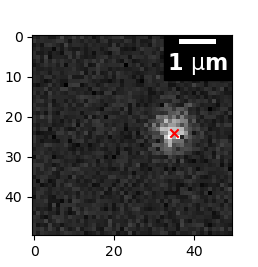
\includegraphics[width=4cm]{MCMC/Figure_1.png}
\end{textblock*}
\begin{textblock*}{4cm}(1.0cm,5cm)
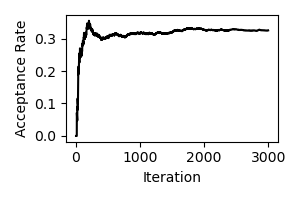
\includegraphics[width=4cm]{MCMC/Figure_2.png}
\end{textblock*}
\begin{textblock*}{9cm}(5cm,1.0cm)
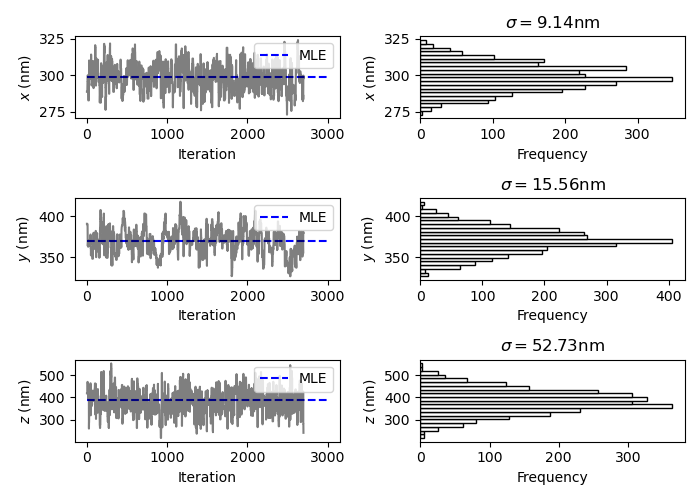
\includegraphics[width=9cm]{MCMC/Figure_3.png}
\end{textblock*}
\begin{textblock*}{13cm}(0.5cm,8cm)
\begin{itemize}
\item Variance of the posterior $P(\theta|\vec{H})$ is a useful particle filter
\item We assume uniform priors on coordinates
\end{itemize}
\end{textblock*}
\end{frame}


\begin{frame}
\frametitle{Direct STORM: The photophysics of rhodamines}

\begin{figure}
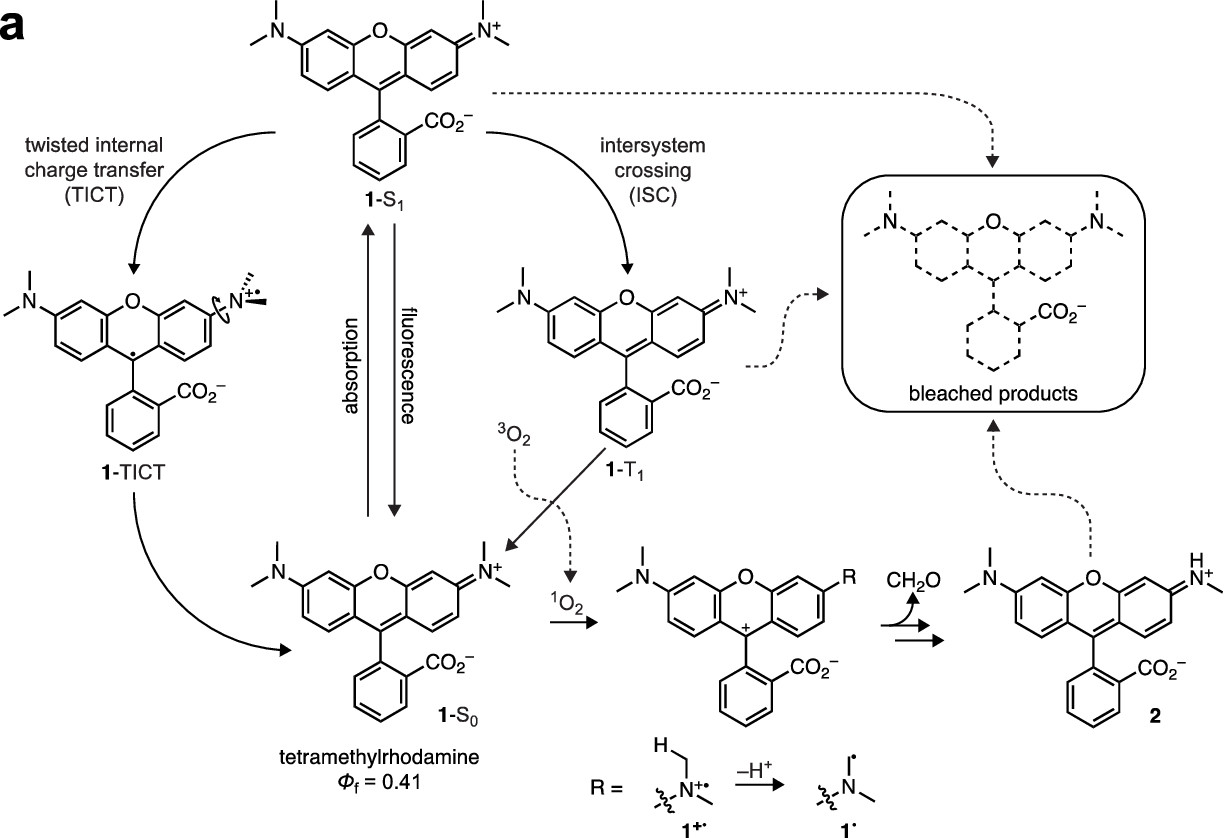
\includegraphics[width=10cm]{Rhodamines.png}
\end{figure}
\begin{itemize}
\item  Reduction of the T1 state yields a dark, long-lived, and stable radical state
\item The reducing agent is usually a primary thiol like cysteamine (MEA)
\end{itemize}
\end{frame}

\begin{frame}{The OFF state of JF646 can be maintained with high laser power}
\begin{textblock*}{11cm}(2.0cm,1.3cm)
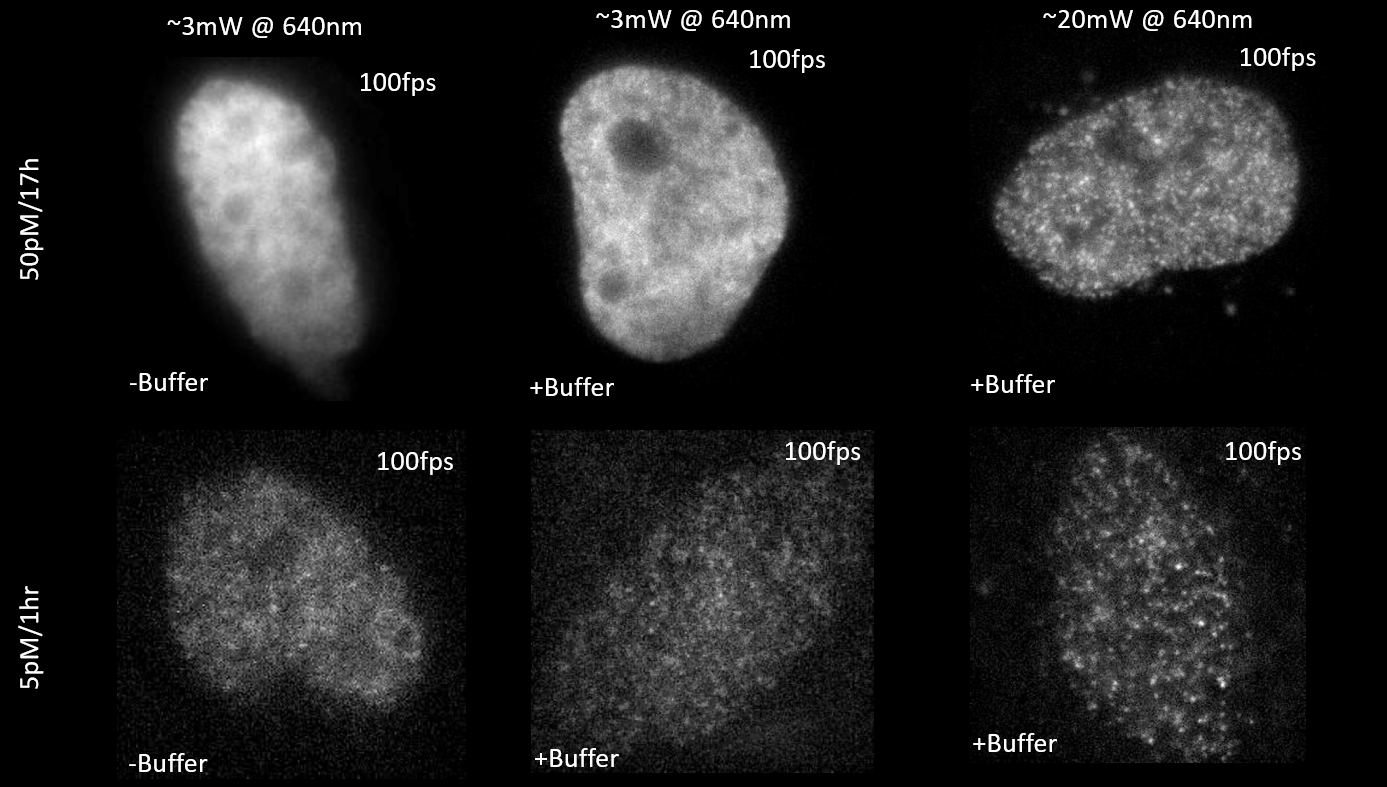
\includegraphics[width=11cm]{Laser.png}
\end{textblock*}
\begin{textblock*}{\textwidth}(0.5cm,8.0cm)
\begin{itemize}
\item Laser power controls the OFF state lifetime
\item Dense labeling is possible for a stable OFF state
\end{itemize}
\end{textblock*}
\end{frame}

\begin{frame}{Fourier ring correlation links spatial and temporal resolution}
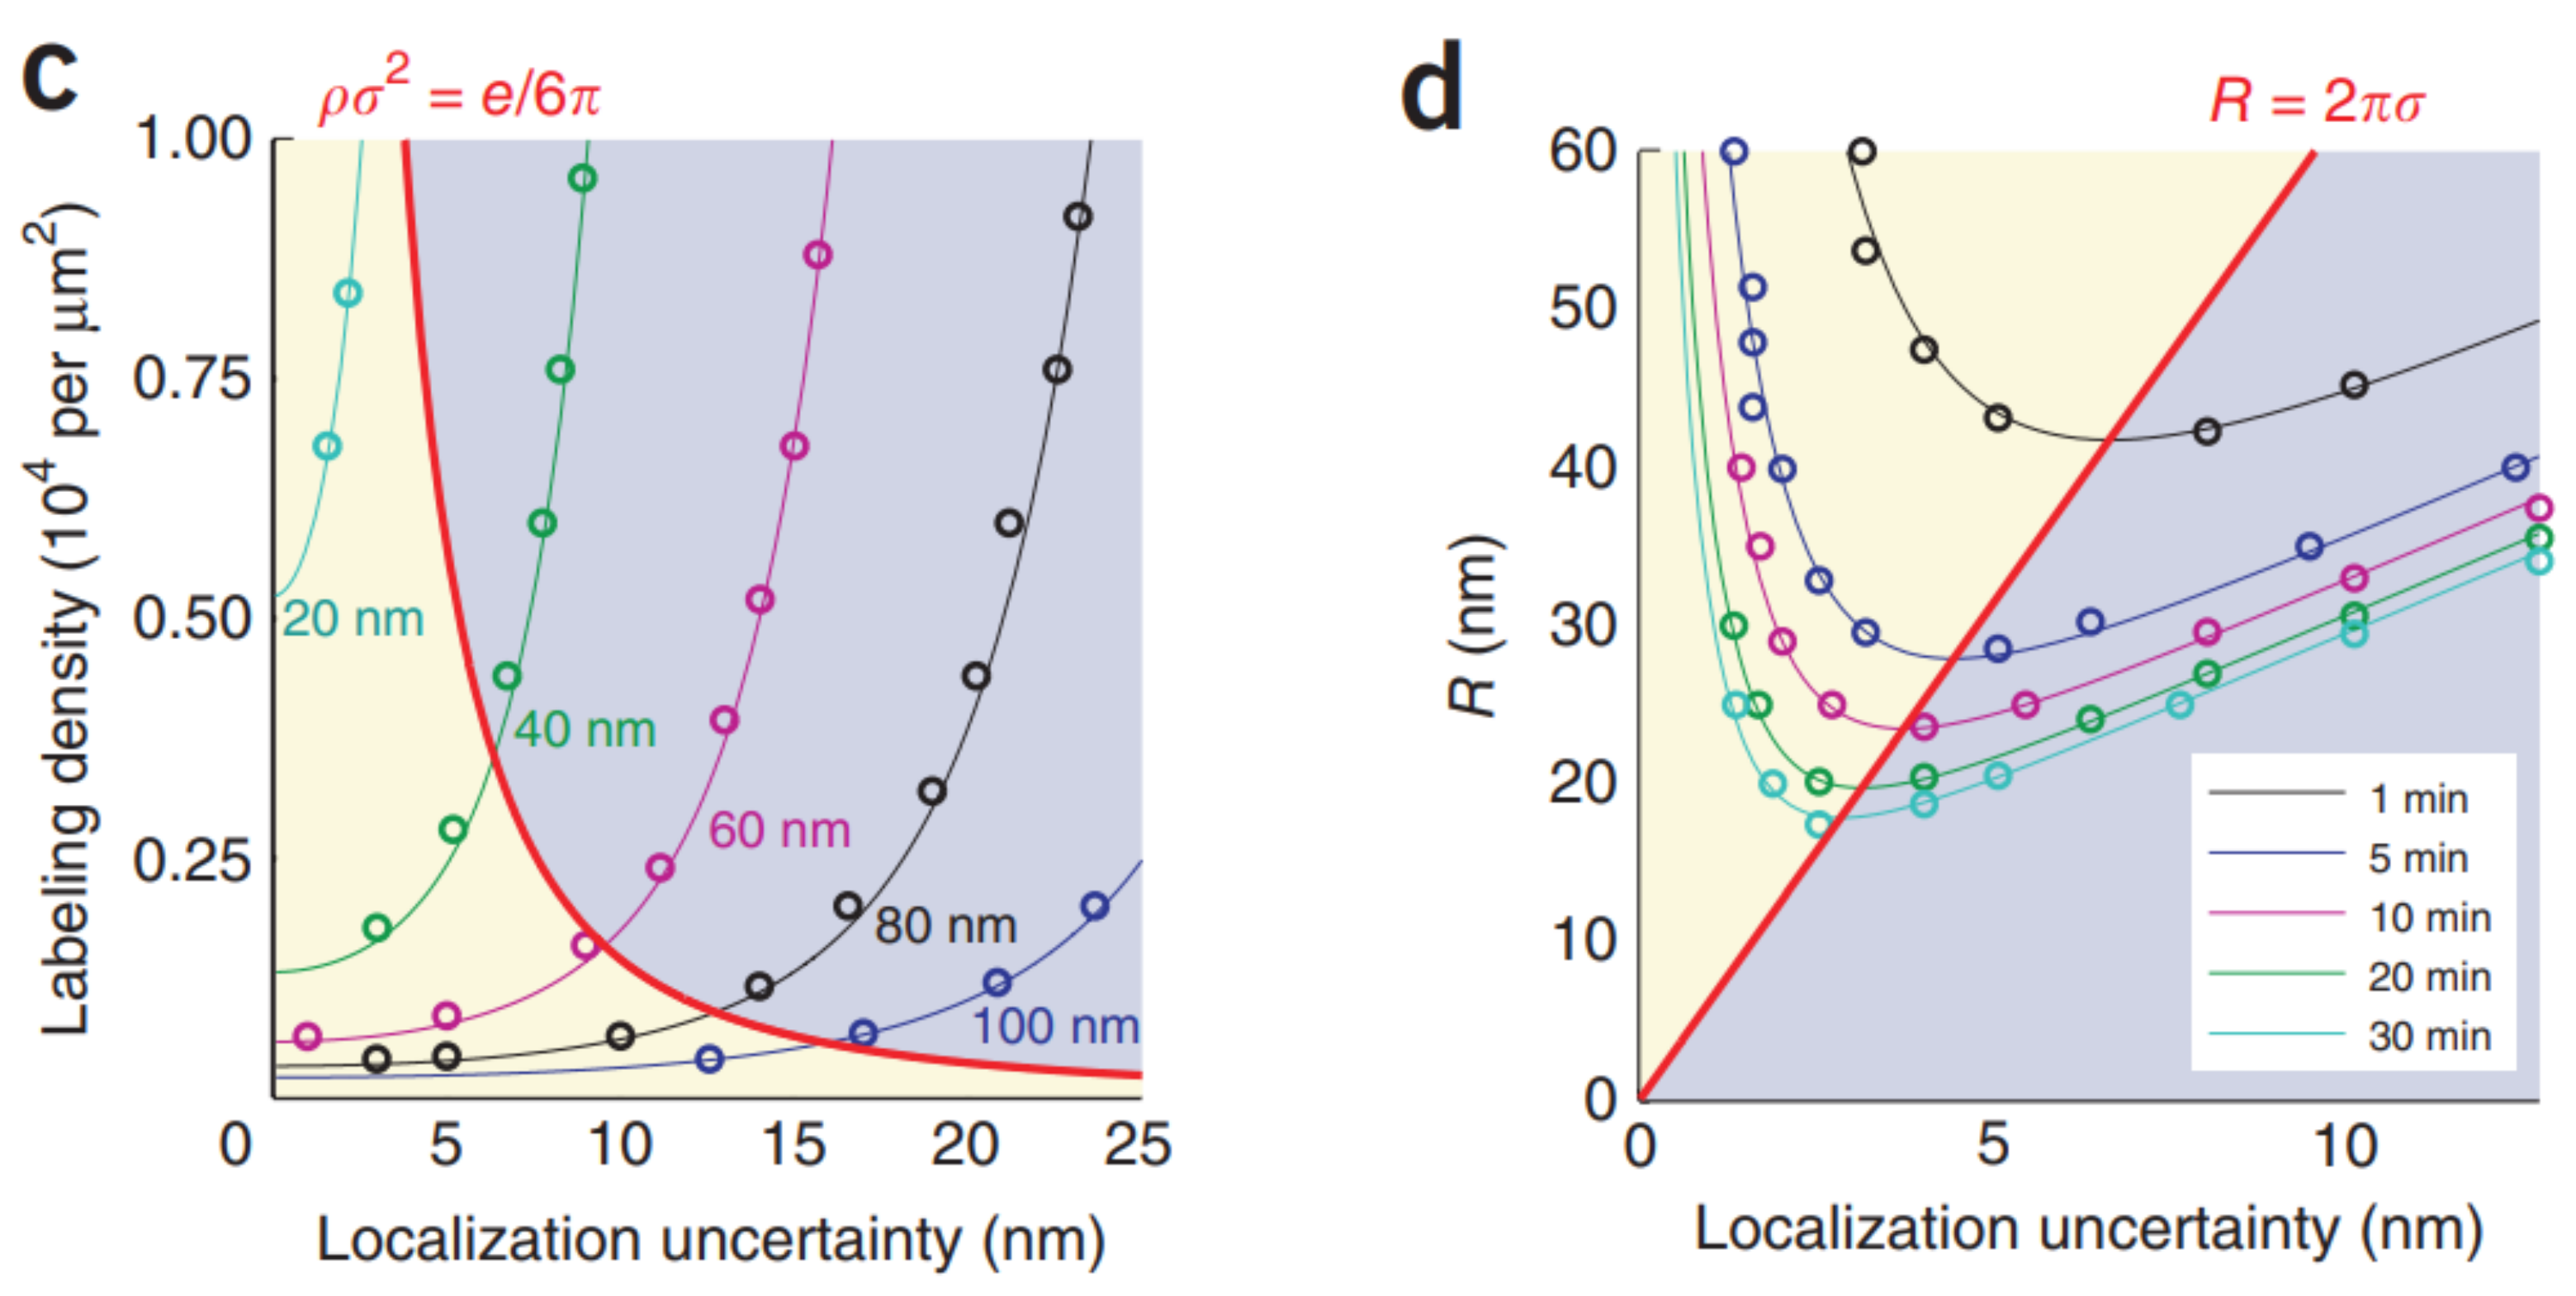
\includegraphics[width=12cm]{Spatial.png}
\textit{Nieuwenhuizen et al. Measuring image resolution in optical nanoscopy. Nature Methods 2013}
\end{frame}


\begin{frame}{Fourier ring correlation links spatial and temporal resolution}
\begin{textblock*}{13cm}(1cm,1.25cm)
\begin{itemize}
\item We can view dSTORM as sampling from a density
\item This is why we use Gaussian kernel density estimation (KDE)
\end{itemize}
\end{textblock*}
\begin{textblock*}{13cm}(1cm,2.75cm)
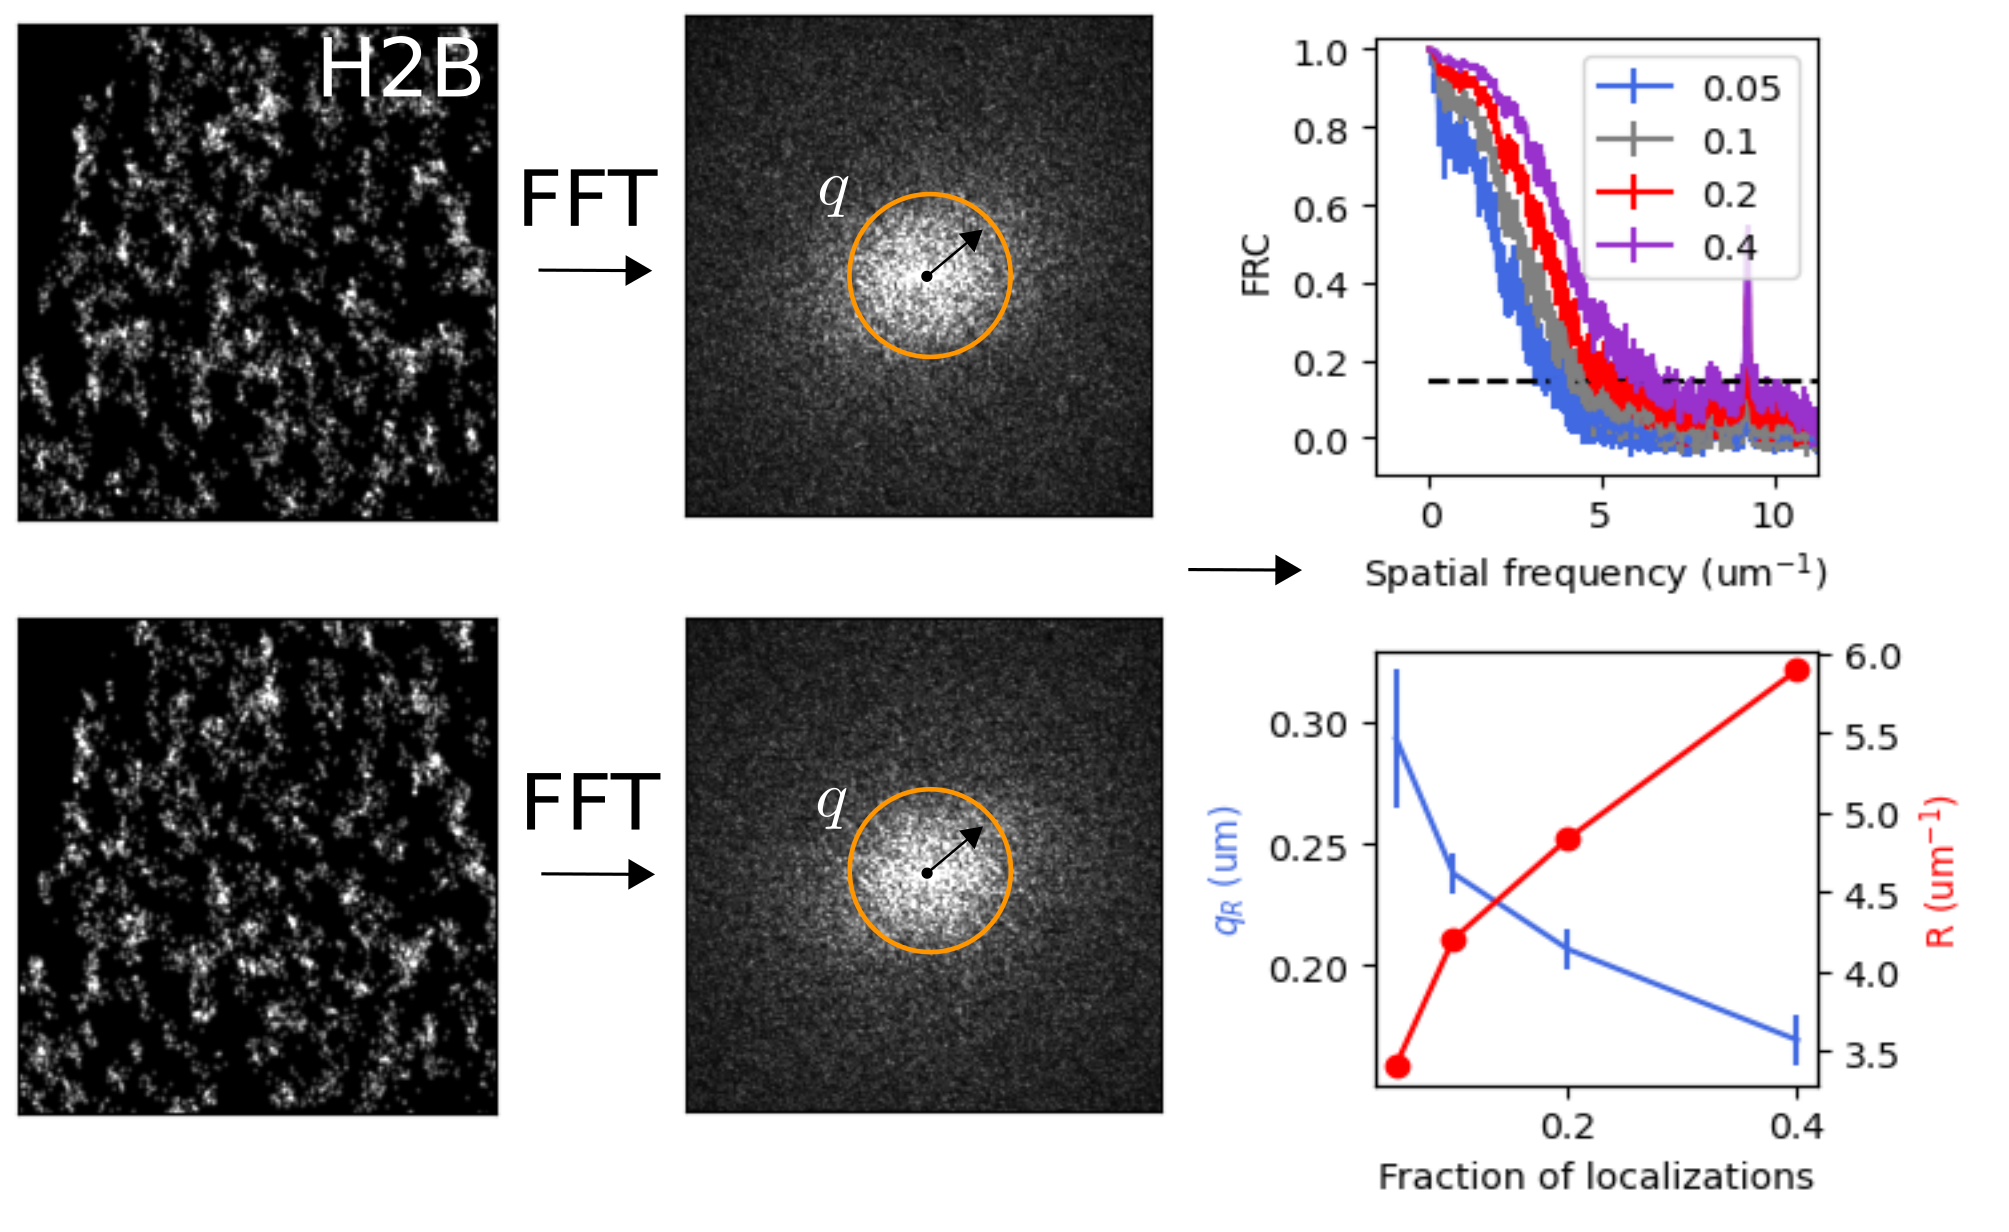
\includegraphics[width=13cm]{FRC.png}
\end{textblock*}
\begin{textblock*}{8cm}(3cm,7.5cm)
\begin{equation*}
\mathrm{FRC}(q) = \frac{\sum_{\vec{q}\in\mathrm{circle}}\tilde{f_{1}}(\vec{q})\tilde{f_{2}}(\vec{q})^{*}}{\sqrt{\sum_{\vec{q}\in\mathrm{circle}}|f_{1}(\vec{q})|^{2}}\sqrt{\sum_{\vec{q}\in\mathrm{circle}}|f_{2}}(\vec{q})|^{2}}
\end{equation*}
\end{textblock*}
\end{frame}

\begin{frame}{Deep learning enables dense localization in two-dimensions}
\begin{textblock*}{10cm}(4.25cm,1.25cm)
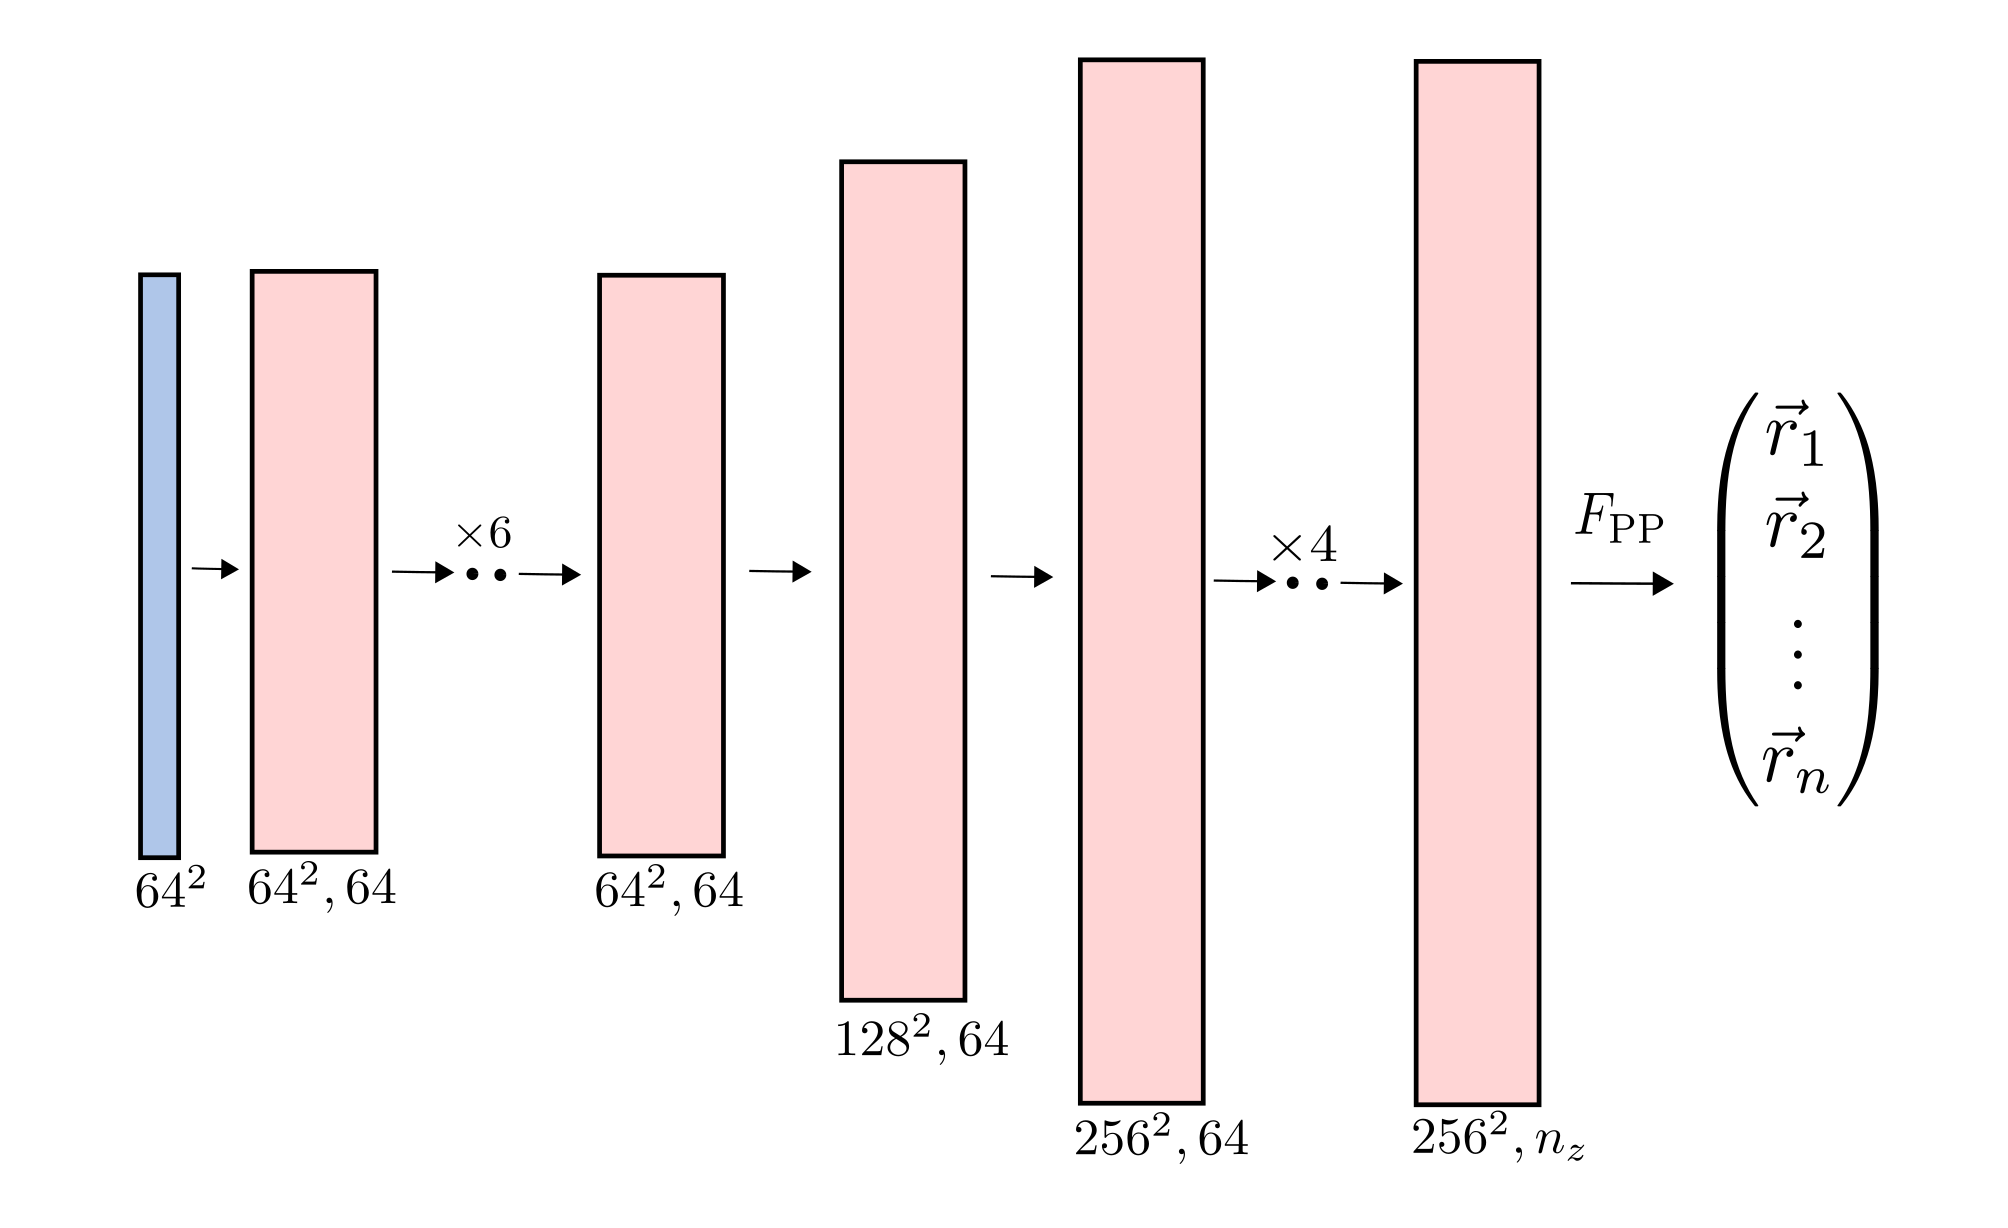
\includegraphics[width=10cm]{DeepSTORM.png}
\end{textblock*}
\begin{textblock*}{2.5cm}(1.5cm,2.75cm)
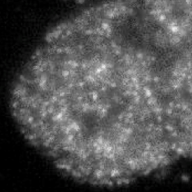
\includegraphics[width=2.5cm]{Laser-Crop.png}
\end{textblock*}

\begin{textblock*}{\textwidth}(1cm,7.5cm)

Localization is cast as semantic segmentation of the high resolution tensor:

\begin{equation*}
\mathcal{L} = \sum_{i,j} \log p_{ij}(\tilde{x}) = \sum_{i,j} \log \frac{\exp(-s_{ij}(\tilde{x}))}{\sum_{x\in\chi} \exp(-s_{ij}(\tilde{x}))}
\end{equation*}

\end{textblock*}

\end{frame}



\begin{frame}{Estimator precision sets the resolution limit in localization microscopy}

\begin{textblock*}{10cm}(1.25cm,1.5cm)
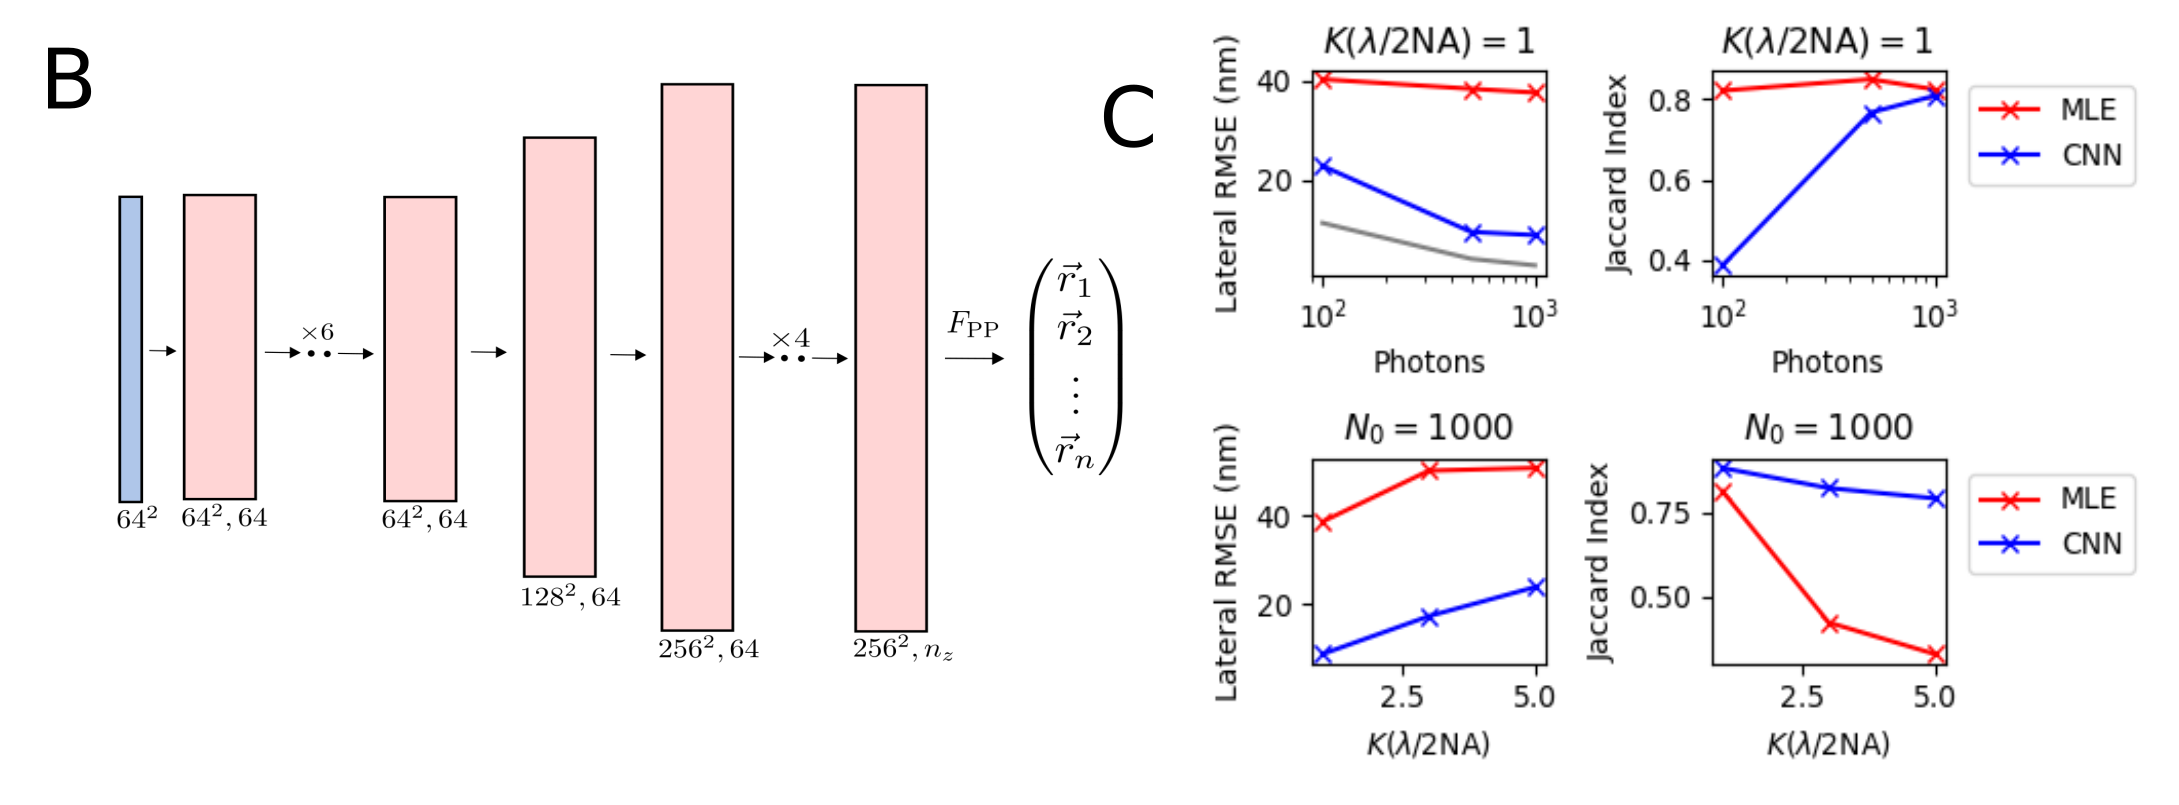
\includegraphics[width=13cm]{PSF2D-Crop.png}
\end{textblock*}
\begin{textblock*}{13cm}(1.25cm,7cm)
\begin{itemize}
\item $K(\lambda/2\mathrm{NA})$ is Ripley's K function at the diffraction limit ($\lambda=640\mathrm{nm}$)
\item Convolutional neural networks (CNNs) approach the Cramer-Rao lower bound (gray)
\end{itemize}
\end{textblock*}

\end{frame}


\begin{frame}{Astigmatism based three dimensional imaging}
\begin{figure}
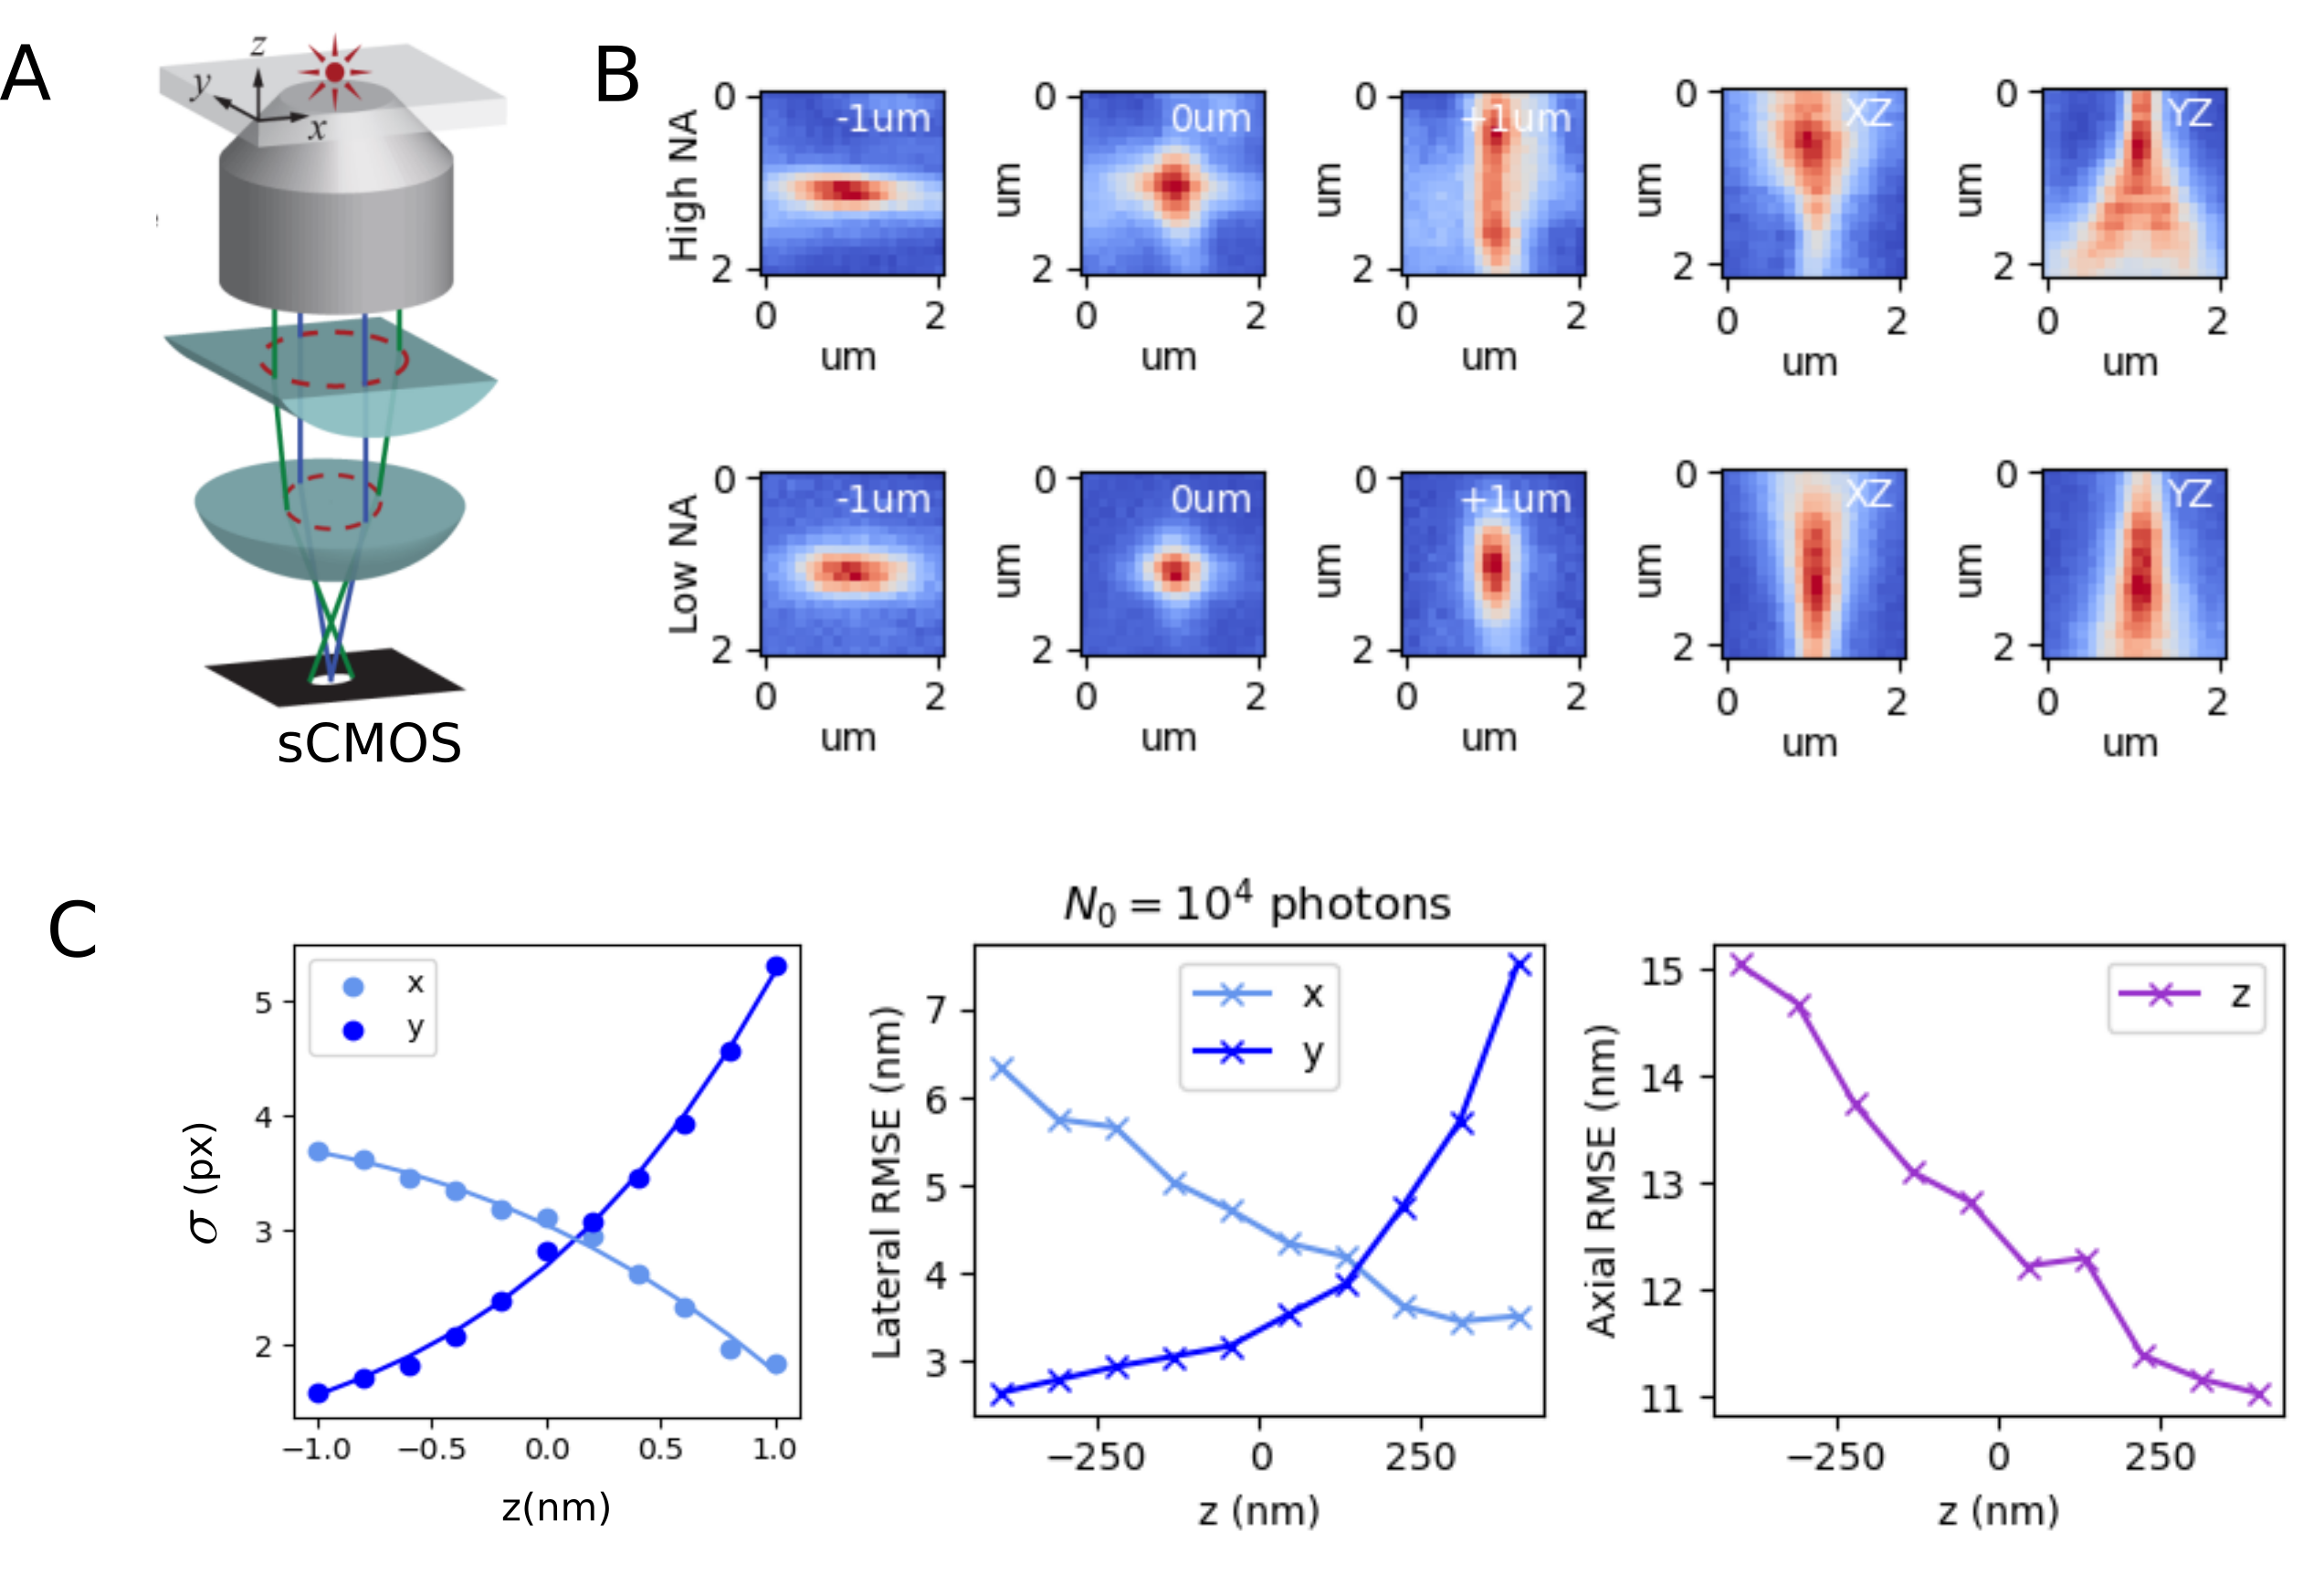
\includegraphics[width=11cm]{Astigmatism.png}
\end{figure}
\begin{itemize}
\item A weak ($f=10$m) cylindrical lens breaks the axial symmetry of the PSF
\end{itemize}
\end{frame}


\begin{frame}{Astigmatism based three dimensional imaging}
\begin{figure}
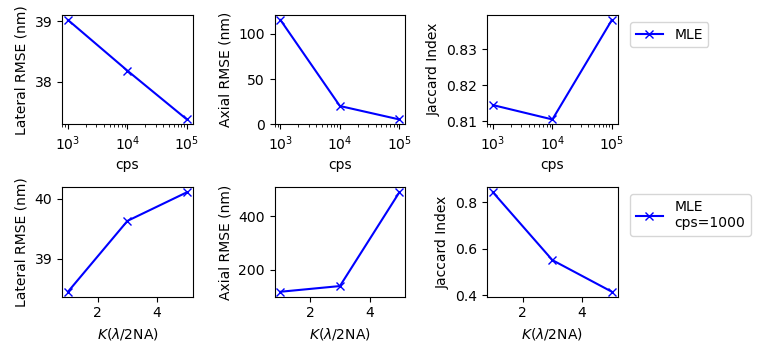
\includegraphics[width=13cm]{PSF3D.png}
\end{figure}
\begin{itemize}
\item $z_{0}\sim U([-0.4,0.4])$ um
\item 3D imaging requires long exposure and sparse emitters for MLE
\item Deep methods may be a suitable choice in future work
\end{itemize}
\end{frame}


\begin{frame}{Chromatin nanodomains in a living Hela cell nucleus}

\begin{textblock*}{13cm}(0.5cm,1.5cm)
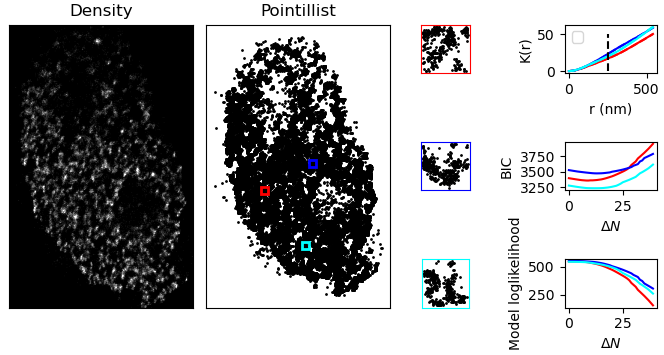
\includegraphics[width=\textwidth]{Cluster.png}
\end{textblock*}

\begin{textblock*}{13cm}(0.5cm,8.0cm)
\begin{itemize}
\item Isotropic Gaussian KDE using 30x30nm bins
\item Closest pairs are fused one at a time, until we minimized the BIC
\item Likelihood is computed under a Gaussian Mixture Model (GMM)
\end{itemize}
\end{textblock*}

\end{frame}

\begin{frame}{Chromatin nanodomains in a living Hela cell nucleus}

\begin{textblock*}{13cm}(0.5cm,1.5cm)
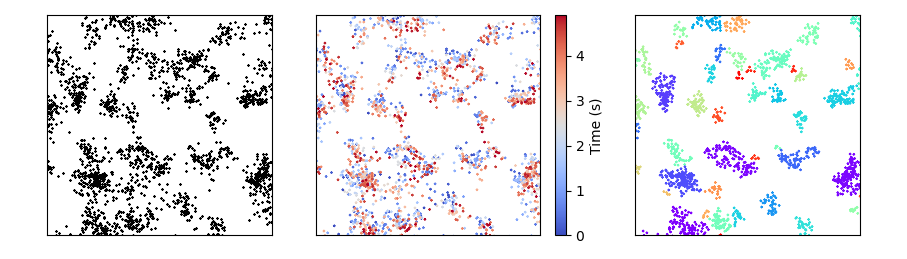
\includegraphics[width=\textwidth]{Cluster2.png}
\end{textblock*}

\begin{textblock*}{13cm}(0.5cm,6.0cm)
\end{textblock*}

\end{frame}

\begin{frame}{Future Aims}

\begin{textblock*}{9cm}(0.5cm,1.5cm)
\begin{itemize}
\item Integrate 2D SMLM and 2D/3D single molecule tracking (Brownian dynamics in a potential)
\item Determine suitable metrics for measuring dynamics of the KDE
\item Publish
\end{itemize}
\end{textblock*}

\begin{textblock*}{3cm}(11.0cm,1.5cm)
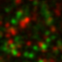
\includegraphics[width=3cm]{Composite.png}
\end{textblock*}

\end{frame}


\end{document}